\chapter{Results}
\label{ch:results}
The experimentation focused on evaluating the performance of various object detection models, particularly YOLO NAS (You Only Look Once Neural Architecture Search), across different configurations. We utilized a range of hyperparameters including epochs, batch sizes, learning rates, and image resolutions to assess their impact on model accuracy and computational efficiency. The experiments were conducted on a dataset of blood cell images, and performance metrics such as Mean Average Precision (mAP) at different IoU thresholds, precision, and recall were measured. 

 



\section{Performance Evaluation of YOLO NAS Model}

We trained multiple variants of YOLO NAS, namely YOLO NAS-S, YOLO NAS-M, and YOLO NAS-L, with varying configurations. The table below summarizes the performance of these models:

\begin{figure}[ht]
    \centering
    \includegraphics[scale=0.8]{Tables/: Performance evaluation metrics of YOLO NAS Model.jpg}
    \caption{Table 4.1 : Performance evaluation metrics of YOLO NAS Model}
    \label{fig:example-01}
\end{figure}
\clearpage
\textbf{Understanding Metrics}:

\textbf{@0.50 Threshold}: This represents the Intersection over Union (IoU) threshold at 0.50, indicating the degree of overlap between predicted and ground-truth bounding boxes. Higher values signify stricter criteria for object detection.

\textbf{@0.50:0.95 Threshold}: This extends the IoU threshold range from 0.50 to 0.95, providing a broader assessment of detection accuracy. Achieving high scores in this metric implies robustness in detecting objects with varying degrees of overlap.

\textbf{Analysis}:

\textbf{YOLO NAS S}:
\begin{itemize}
    \item Achieved a moderate mAP@0.50 of 0.1111 and mAP@0.50:0.95 of 0.0701.
    \item Precision@0.50 was 0.0345, indicating a lower precision at the 0.50 
IoU threshold.
    \item  Recall@0.50:0.95 was 0.68, suggesting relatively better performance in capturing objects with a broader range of IoU thresholds.
\end{itemize}

\textbf{YOLO NAS M}:
\begin{itemize}
    \item Demonstrated superior performance with a higher mAP@0.50 of 0.0978 and mAP@0.50:0.95 of 0.0613.
    \item Precision@0.50 and Precision@0.50:0.95 were notably better at 0.0469 and 0.0333, respectively.
    \item Achieved a commendable Recall@0.50:0.95 of 0.6845, indicating robustness in detecting objects with varying overlaps.
\end{itemize}

\textbf{YOLO NAS L}:
\begin{itemize}
    \item Showcased competitive performance with a mAP@0.50 of 0.1042 and mAP@0.50:0.95 of 0.0696.
    \item Precision@0.50 and Precision@0.50:0.95 were decent at 0.0542 and 0.0416, respectively.
    \item Achieved a high Recall@0.50:0.95 of 0.7082, indicating strong detection capabilities at stricter IoU thresholds.
\end{itemize}

\textbf{Conclusion}:

YOLO NAS M outperformed both YOLO NAS S and YOLO NAS L across all metrics.

It achieved higher mAP scores and demonstrated superior precision and recall rates, especially at stricter IoU thresholds (@0.50:0.95).

\begin{figure}[ht]
    \centering
    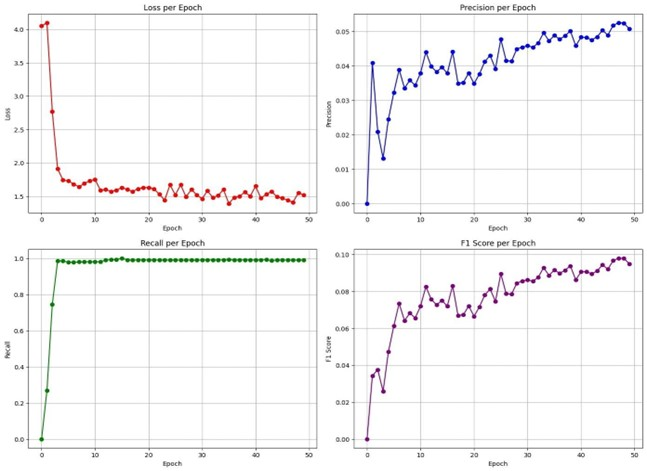
\includegraphics[scale=1.0]{figures/Training Metric Overview.jpg}
    \caption{Figure 4.1 : Training Metrics Overview per Epoch}
    \label{fig:example-01}
\end{figure}


\begin{itemize}
    \item The robust performance of YOLO NAS M makes it the most suitable choice for tasks requiring accurate and reliable object detection.
\end{itemize}





\clearpage
\section{Summary }

The results indicate that the choice of hyperparameters significantly influences the performance of YOLO NAS models. For instance, increasing the batch size led to faster convergence but often resulted in out-of-memory (OOM) errors, particularly for larger models such as YOLO NAS-L. Similarly, adjusting the learning rate and image resolution impacted both the accuracy and speed of object detection. We observed that smaller image resolutions generally led to faster inference times but compromised detection accuracy, especially for smaller objects like blood cells.

Overall, YOLO NAS models demonstrated competitive performance compared to standard YOLO variants, achieving high precision and recall rates across different configurations. However, there is a trade-off between model accuracy and computational efficiency, highlighting the importance of selecting appropriate hyperparameters based on specific application requirements.











